\documentclass[10pt]{article}
\usepackage[letterpaper,margin=0.75in]{geometry}
\usepackage{times}
\usepackage{microtype}
\usepackage{graphicx}
\usepackage{booktabs}
\usepackage[font=small,labelfont=bf,skip=3pt]{caption}
\usepackage[hidelinks]{hyperref}
\usepackage{enumitem}
\usepackage{titlesec}
\titlespacing*{\section}{0pt}{6pt}{2pt}
\titleformat*{\section}{\large\bfseries}
\setlist{nosep,leftmargin=1.2em}
\setlength{\parskip}{3pt}
\setlength{\parindent}{0pt}

\title{\vspace{-2.2em}\textbf{Counterfactual simulation on a budget:\\a model of whether judgments in crowded scenes}}
\author{Jadon Zhu \quad \small\texttt{jadonjzhu@gmail.com} \quad \small\url{https://github.com/JadonJZhu/budgeted-sim}}
\date{\vspace{-2.2em}}

\begin{document}
\maketitle

\section*{The question}
Lu, Bechlivanidis and Gerstenberg (CogSci 2026) found that the whether predictions of the counterfactual simulation model (CSM; Gerstenberg et al., 2021) drift away from people as billiard scenes get crowded, while its how predictions stay accurate. In crowded scenes people's whether and how ratings become nearly the same, even in videos built so that the true answers differ. The paper reads this as people giving up costly simulation for a contact-tracing shortcut, but does not model the shortcut. The CSM's own noise, which perturbs the one ball A hit first, does not explain it. In the 9-ball whether-only video (Figure~\ref{fig:nine}), people's mean flipped whether rating is 20 while the CSM says 96, and the CSM stays between 86 and 100 at every noise level the paper fits (0 to 5 degrees). Noise on every ball whose path changes, growing with the number of balls, can fit this video; we test that version below.

\begin{figure}[h]
\centering
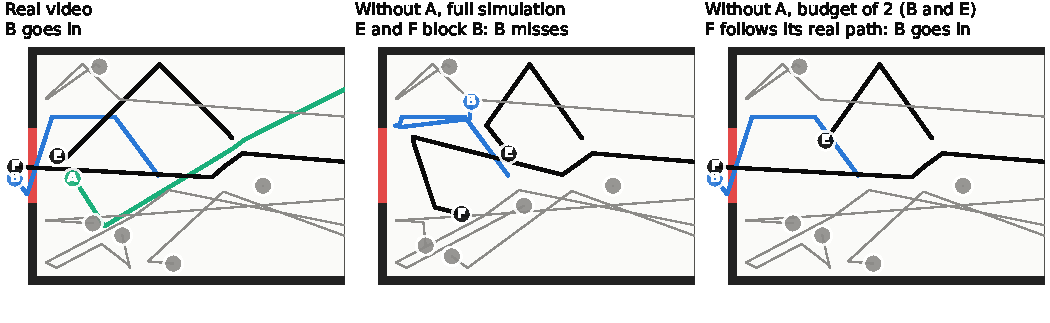
\includegraphics[width=\textwidth]{figures/nine_ball.pdf}
\caption{The 9-ball whether-only video. A sends E and F away and never touches B. Without A, a full simulation sends E and F into B and B misses. Re-simulating only B and E, with F on the path A really sent it on, leaves B's way clear, which matches people's answer.}
\label{fig:nine}
\end{figure}

\section*{The budget model}
We propose that when people imagine the scene without A, they re-simulate only $k$ balls, B first, and let every other ball move along the path it really took. Replayed balls still push the balls being re-simulated, but are never pushed off their own paths. Because the replayed balls already carry A's effects, with $k=1$ B's imagined path can change only if A hit B directly, and the model says A mattered only when that hit decided whether B went in. A's influence through chains of other balls drops out, which is the information people seem to lose in crowded scenes. With every ball in the budget, the model is the CSM. This fits Balaban and Ullman (2025), who found that people can update only about one moving object at a time in imagination. Lu et al.\ cite that result as a reason simulation should fail; the budget makes it part of the model. The other balls in the budget are chosen by a rule that uses only what the video shows. We tested three: the balls A touched, the balls that touched B, and the balls that came closest to B's path.

\section*{Results on the existing data}
We wrote our own simulator from the settings in the paper and code (the repository has no licence, so we did not reuse its code). It matches the original's noise-free whether outcome and how answer in all 20 videos. At $\theta=1.9$ it correlates with mean whether ratings at $r=.670$ over 20 seeds (range .664 to .679); the original code run the same way gives .674 (range .667 to .682).

Every model maps its prediction to the rating scale with a fitted line and is scored on each video after fitting the other 19 (Table~\ref{tab:loo}). The budget model fits best, with $k=2$ filled by B and the first ball A hit; that setting was chosen in all 20 folds, against budgets of 1 or 3 and against the full CSM. On held-out error alone, though, a budget of 1 does as well (18.2), so the existing data do not pin down $k$. Its error does not grow with the number of balls (Figure~\ref{fig:err}; slope $-0.8$ points per ball, 95\% interval $-2.2$ to $0.6$).

\begin{minipage}[t]{0.47\textwidth}
\vspace{0pt}
\centering
\captionof{table}{Leave-one-video-out fit to mean flipped whether ratings (RMSE in rating points).}
\label{tab:loo}
\small
\begin{tabular}{lcc}
\toprule
Model & RMSE & $r$ \\
\midrule
Budget, $k=2$ (ours) & 18.2 & .80 \\
Crowding noise ($\theta$ grows with balls) & 22.5 & .67 \\
How only & 24.3 & .59 \\
Full CSM & 25.1 & .55 \\
\bottomrule
\end{tabular}
\end{minipage}\hfill
\begin{minipage}[t]{0.49\textwidth}
\vspace{0pt}
\centering
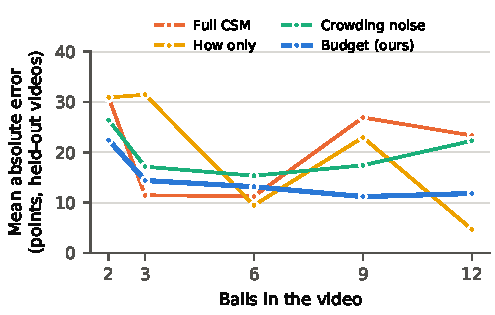
\includegraphics[width=\linewidth]{figures/error_by_balls.pdf}
\captionof{figure}{Error on held-out videos by number of balls.}
\label{fig:err}
\end{minipage}

\medskip
The advantage is not decisive. Resampling participants 1,000 times, the budget model beats the CSM in 96\% of resamples (95\% interval of the RMSE gap $-10.8$ to $+0.6$), crowding noise in 81\% and how only in 87\%. We fixed a 95\% interval excluding zero as the bar before fitting, and the result does not clear it: with 20 videos, the existing data cannot separate these models. Fitting each participant separately, the budget model fits 34\% of people best (how only 28\%, crowding noise 28\%, CSM 10\%), and the best budget across all 50 people is 1 ball for 13, 2 for 25 and 3 for 12. For cause ratings, the authors' proposed certainty-weighted combination of whether and how predicts better with the budget model's whether answers than with the CSM's (held-out RMSE 16.7 vs.\ 18.3; the whether settings themselves were fit on all 20 videos).

\section*{A test that separates the models}
We generated 500,000 random scenes in the style of the originals (3 to 9 balls), kept the 37,167 that meet the original videos' constraints (B goes in, 7 to 13 seconds, every collision on screen, no two collisions close in time and place, no near-touch that a viewer could mistake for contact), and selected test scenes by fixed rules, so none was picked by hand. A scene qualifies when two models' predicted probabilities differ by at least 40 points at every setting the existing data cannot rule out: budgets of 1 to 3 balls, and every noise level on the paper's grid (0 to 5 degrees) whose fit is inside the 95\% bootstrap interval of the best. At the fitted rating scales this is 41 to 47 rating points on average for the three which-model kinds, against a measurement uncertainty of at most $\pm 12$ points for a video's mean rating in the original data.

\begin{center}
\small
\begin{tabular}{lcccccc}
\toprule
Kind of scene & $n$ & Budget & Full CSM & Crowding & How only \\
\midrule
Clear the way: A removes a ball that would have blocked B & 8 & 25 & 73 & 66 & 56 \\
Budget vs.\ crowding noise & 8 & 25 & 66 & 69 & 50 \\
Hit but no difference: A hits B, B would have gone in anyway & 8 & 25 & 16 & 16 & 66 \\
Budget of 1 vs.\ 2, and 2 vs.\ 3 (half in each direction) & 8 & 25 or 83 & 48 & 56 & 66 \\
Original videos as anchors & 4 & 54 & 62 & 41 & 45 \\
\bottomrule
\end{tabular}

\smallskip
\footnotesize Mean predicted rating (flipped whether, 0 to 100) of each model at its best fit to the existing data.
\end{center}

Across the 36 scenes, no crude cue (A's closest approach to B, number of collisions or balls, A passing near B's path) correlates with any model's disagreement with the budget model above $|r| = .3$ (largest .26). We simulated studies of 50 people in which each fake person copies one real participant's slider scale and noise. The generating model won all 200 studies and its budget size was recovered in all 200, for every model and for $k = 1$, 2 and 3. A population mixing budgets in the proportions of the per-person fits was identified as a budget population every time, with $k = 2$ in 199 of 200. The 36 scenes (about 27 minutes), rendered videos, every model's prediction at every setting, and a pre-registration-style plan with pass and fail lines are in the repository.


\section*{References}
\small
Balaban, H., \& Ullman, T. D. (2025). The capacity limits of moving objects in the imagination. \textit{Nature Communications}.\\
Gerstenberg, T., Goodman, N. D., Lagnado, D. A., \& Tenenbaum, J. B. (2021). A counterfactual simulation model of causal judgments for physical events. \textit{Psychological Review}.\\
Lu, X., Bechlivanidis, C., \& Gerstenberg, T. (2026). Causal judgments in complex situations. \textit{CogSci 2026}. Materials: \url{https://github.com/cicl-stanford/complex_causation_cogsci2026}.

\end{document}
